\ylDisplay{Kondensaator} % Ülesande nimi
{Jaan Kalda} % Autor
{lahtine} % Voor
{2017} % Aasta
{G 7} % Ülesande nr.
{8} % Raskustase
{
% Teema: Elektrostaatika
\ifStatement
\begin{wrapfigure}[5]{r}{0.35\linewidth}
	\vspace{-13pt}
	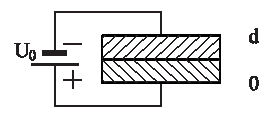
\includegraphics[width=\linewidth]{2017-lahg-07-res-cap2.pdf}
\end{wrapfigure}

Plaatkondensaator mahtuvusega $C$ omab plaatidevahelist kaugust $d$. Plaatide vahele asetatakse kaks dielektrilist plaati paksusega $d/2$. Ühe plaadi dielektriline läbitavus on $\varepsilon$, teisel $2\varepsilon$. Milline on nüüd kondensaatori mahtuvus? Milline laeng on plaatide eralduspinnal, kui kondensaatorile rakendatakse pinge $U_0$?
\fi


\ifHint
Mahtuvuse leidmiseks võib kondensaatorit vaadelda kui kahte jadamisi ühendatud dielektrikuga kondensaatorit. Selleks asetame mõttelise metallplaadi dielektrilise kihi eralduspinnale. Eralduspinna laengu leidmiseks võib rakendada Gaussi teoreemi mõttelise \enquote{karbi} jaoks, mis hõlmab piirpinda.
\fi


\ifSolution
Vaatleme kahe dielektrikuga kondensaatorit kui kahte järjestikku ühendatud plaatkondensaatorit. Selleks asetame mõttelise metallplaadi dielektriliste kihtide eralduspinnale. Ühel kondensaatoril on seal laeng $+q$, teisel $-q$, seega vaba laeng on mõttelisel metallplaadil null (nii nagu vaja, sest tegelikult seal ju metallplaati pole). Algse dielektrikuta kondensaatori mahtuvus $C=\varepsilon_0S/d$. Mõtteliste kondensaatorite mahtuvused on $C_1=S\varepsilon_0\varepsilon/(d/2)=2\varepsilon C$ ja $C_2=S\varepsilon_02\varepsilon/(d/2)=4\varepsilon C$, seega summaarse mahtuvuse pöördväärtus $C'=C_1C_2(C_1+C_2)=\frac 43\varepsilon C$ (1 p).

Dielektrikuga kondensaatori mahtuvus erineb dielektrikuta kondensaatori mahtuvusest, sest lisaks vabale laengule $q$ metallplaadil on veel dielektriku pinnal vastasmärgiline dielektriku polarisatsioonist tingitud (dielektrikust mitte-eraldatav) laeng $-q'$. Summaarne laeng $Q=q-q'$ on selline, nagu on antud pinge puhul samasugusel, ilma dielektrikuta kondensaatoril. Olgu ühe mõttelise kondensaatori kogulaeng (vaba laeng + dielektriku laeng) $Q_1=q-q_1'$ ja teisel $Q_2=q-q_2'$, siis sellel plaadil, mis jääb dielektrikute eralduspinnale, on kondensaatori plaatide laengumärke arvestades kogulaeng $Q_1-Q_2=q_2'-q_1'$. Seega, dielektrikute eralduspinnal oleva kogulaengu $q_2'-q_1'$ saame leida, kui selliste dielektrikuta kondensaatorite laengute vahe, mille pinge võrdub vastavale dielektrikukihile langeva pingega. 

Mõttelistel kondensaatoritel on ühesugune laeng, seose $U=q/C$ tõttu on pinge pöördvõrdeline mahtuvusega, st ühele poole (kus dielektriline läbitavus  on $\varepsilon$) langeb pinge $2U_0/3$ ja teisele poole (kus dielektriline läbitavus on $2\varepsilon$) $U_0/3$. Kui dielektriku kihti ei oleks, siis oleks kummagi mõttelise kondensaatori mahtuvus $2C$. Seega laeng mõttelistel kondensaatoritel oleks vastavalt $Q_1=4U_0C/3$ ja $Q_2=2U_0C/3$, mistõttu kogulaeng dielektrikute eralduspinnal $q'=Q_1-Q_2=2CU_0/3$.
\vspace{0.5\baselineskip}

\emph{Alternatiivne lahendus}\\
Olgu kondensaatori plaadil laeng $q$, siis Gaussi teoreemist kondensaatori plaadi jaoks saame seose $SD=q$, millest $D=q/S$. Dielektrikute eralduspinnal on $D$-vektori normaalkomponent pidev, seega piirkonnas, kus dielektriline läbitavus on $\varepsilon$, on $E_1=D/\varepsilon\varepsilon_0$, teises piirkonnas $E_2=D/2\varepsilon\varepsilon_0$. Järelikult $U_0=E_1\frac d2+E_2\frac d2=(Dd/2\varepsilon\varepsilon_0)(1+\frac 12)=\frac 34Qd/\varepsilon\varepsilon_0S$, millest $C'\equiv Q/U_0=\frac 43\varepsilon\varepsilon_0S/d=\frac 43C\varepsilon$. Laengu piirpinnal $q'$ leiame Gaussi teoreemi abil mõttelise \enquote{karbi} jaoks, mis hõlmab piirpinda: $q'=(E_1-E_2)\varepsilon_0S=DS/2\varepsilon=q/2\varepsilon=U_0C'/2\varepsilon=\frac 23CU_0$.
\fi


\ifEngStatement
% Problem name: Capacitor
\begin{wrapfigure}[5]{r}{0.35\linewidth}
	\vspace{-13pt}
	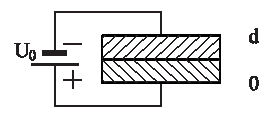
\includegraphics[width=\linewidth]{2017-lahg-07-res-cap2}
\end{wrapfigure}
The distance between the plates of a parallel plate capacitor is $d$. The capacitor’s capacity is $C$. Two dielectric plates of width $d/2$ are placed between the capacitor’s plates. The relative permittivity of one plate is $\varepsilon$, the other’s is $2\varepsilon$. What is the capacity of the capacitor now? What is the charge at the interface between the two plates if a voltage $U_0$ is applied to the capacitor?
\fi


\ifEngHint
To find the capacitance the capacitor can be looked at as two separate capacitors with dielectrics that are connected in series. For this we place the metal plate on the separation surface of the imaginary dielectric layer. To find the charge of the interface you can use the Gauss theorem for an imaginary "box" that includes the interface.
\fi


\ifEngSolution
Let us observe the capacitor with two dielectrics as two parallel plate capacitors connected in series. For that we place an imaginary metal plate on the interface of the dielectric layers. One of the capacitors has a charge $+q$ there, the other one $-q$, therefore the free charge on the imaginary metal plate is zero (as it is needs to be because the metal plate is not actually there). The capacitance of the initial capacitor without a dielectric is $C=\varepsilon_0S/d$. The capacitances of the imaginary capacitors are $C_1=S\varepsilon_0\varepsilon/(d/2)=2\varepsilon C$ and $C_2=S\varepsilon_02\varepsilon/(d/2)=4\varepsilon C$, therefore the inverse of the total capacitance is $C'=C_1C_2(C_1+C_2)=\frac 43\varepsilon C$. \\
The capacitance of a capacitor with a dielectric differs from the capacitance of the capacitor without a dielectric because in addition to the free charge $q$ on the metal plate there is also an opposite charge $-q'$ (non-separable from the dielectric) on the surface of the dielectric due to the polarization of the dielectric. The total charge $Q=q-q'$ is such that an identical capacitor without a dielectric would have on the same voltage. Let the total charge (free charge + dielectric’s charge) of one the imaginary capacitors be $Q_1=q-q_1'$ and the other’s $Q_2=q-q_2'$, then on the plate that stays on the interface of the dielectrics the total charge is $Q_1-Q_2=q_2'-q_1'$, for which the charge symbols of the capacitor’s plates were also taken into account. Therefore we can find the total charge $q_2'-q_1'$ on the interface of the dielectrics as a charge difference of such capacitors without a dielectric that have a voltage equal to the voltage applied to a respective dielectric layer.\\
The imaginary capacitors have the same charge. Due to the relation $U=q/C$ voltage is reversely proportional to capacitance, meaning that one side (where the dielectric permittivity is $\varepsilon$) is applied with a voltage $2U_0/3$ and the other side (where the dielectric permittivity is $2\varepsilon$) with $U_0/3$. If there was no dielectric layer then both of the imaginary capacitors would have a capacitance $2C$. Therefore the charge on the imaginary capacitors would be respectively $Q_1=4U_0C/3$ and $Q_2=2U_0C/3$ which is why the total charge on the interface of the dielectrics is $q'=Q_1-Q_2=2CU_0/3$.\\

\emph{Alternative solution}\\
Let there be a charge $q$ on the capacitor’s plate, then from the Gauss’s law we get a relation $SD=q$ for the capacitor’s plate, where $D=q/S$. On the interface of the dielectrics the normal component of the $D$-vector is continuous therefore in the region where the dielectric permittivity is $\varepsilon$ there is $E_1=D/\varepsilon\varepsilon_0$, in the other region $E_2=D/2\varepsilon\varepsilon_0$. Thus, $U_0=E_1\frac d2+E_2\frac d2=(Dd/2\varepsilon\varepsilon_0)(1+\frac 12)=\frac 34Qd/\varepsilon\varepsilon_0S$, from which $C'\equiv Q/U_0=\frac 43\varepsilon\varepsilon_0S/d=\frac 43C\varepsilon$. With the help of the Gauss’s law, at the interface $q'$ of the charge we find the following relation for an imaginary “box” that includes the interface: $q'=(E_1-E_2)\varepsilon_0S=DS/2\varepsilon=q/2\varepsilon=U_0C'/2\varepsilon=\frac 23CU_0$.
\fi
}